\chapter{Methodisches Vorgehen und Systemkonzeption}

\section{Forschungsdesign und Untersuchungslogik}

Zur Beantwortung der Forschungsfragen wird ein mehrstufiges Untersuchungsdesign verwendet,
das die Analyse der Repräsentationen von der späteren Bewertung des prototypischen
Klassifikationssystems trennt. Die eingesetzten BERT- und RoBERTa-Basisencoder wurden bereits
allgemein selbstüberwacht vortrainiert. Zunächst wird untersucht, welchen zusätzlichen Beitrag
eine task-adaptive selbstüberwachte Anpassung der URL- und HTML-Text-Repräsentationen
leistet. Erst anschließend werden auf Systemebene der Informationsumfang, die multimodale
Fusion und die kaskadierte Verarbeitung variiert. Dadurch lassen sich Veränderungen der
Repräsentationen getrennt von später eingeführten Architekturkomponenten untersuchen.

Die vier Forschungsfragen folgen dieser Reihenfolge. FF1 vergleicht R0, RU, RT und RUT
unter konstant gehaltenen Downstream-Bedingungen. FF2 erweitert den Vergleich über sieben
verschachtelte Labelbudgets und zwei Downstream-Probes. FF3 prüft, ab welchem reduzierten
Labelbudget RUT das Leistungsniveau vollständig mit 200.000 Labels trainierter Referenzen
über alle fünf Evaluationsbedingungen erreicht. FF4 untersucht anschließend auf Systemebene zunächst den zusätzlichen Beitrag von
HTML-Text, DOM und Gating zur Erkennungsleistung. Darauf aufbauend wird geprüft, wie das
resultierende multimodale Vollsystem innerhalb einer URL-first-Kaskade gestuft eingesetzt
werden kann und welche Auswirkungen dies auf Klassifikationsleistung und Inferenzaufwand hat.

\begin{table}[htbp]
\centering
\small
\setlength{\tabcolsep}{4pt}
\renewcommand{\arraystretch}{1.12}
\caption{Untersuchungsstufen und Funktion im Untersuchungsdesign.}
\label{tab:untersuchungslogik}
\begin{tabular}{p{0.09\textwidth}p{0.32\textwidth}p{0.47\textwidth}}
\hline
\textbf{Stufe} & \textbf{Vergleich} & \textbf{Zweck} \\
\hline
FF1 & R0, RU, RT, RUT & Zusätzlicher Beitrag der task-adaptiven URL- und Textrepräsentation \\
FF2 & 2k--200k Labels; Linear Probe und MLP & Lernverhalten bei unterschiedlicher gelabelter Supervision \\
FF3 & RUT$_B$ gegen R0@200k und TF-IDF/XGBoost@200k & Erreichen des Leistungsniveaus vollständig trainierter Referenzen \\
FF4 & URL $\rightarrow$ DUAL $\rightarrow$ TRI $\rightarrow$ Gated $\rightarrow$ Kaskade & Zusätzlicher Systembeitrag und gestufte Systemverarbeitung \\
\hline
\end{tabular}
\end{table}

Die Untersuchungsstufen greifen damit unterschiedliche Aspekte derselben betrieblichen
Problemstellung auf. Die Low-FPR-Evaluation berücksichtigt die Qualität der
Klassifikationsentscheidung bei begrenztem Fehlalarmniveau. Die Labelbudgetanalyse untersucht,
wie viel gelabelte Downstream-Supervision zum Erreichen eines festgelegten Leistungsniveaus
erforderlich ist. Die nachgelagerte Systemanalyse bestimmt zunächst, welchen zusätzlichen
Beitrag HTML-Text, DOM und Gating zur Erkennungsleistung leisten. Erst auf Basis dieses
leistungsstarken Vollsystems wird anschließend untersucht, wie eine URL-first-Kaskade die
Verarbeitungstiefe instanzabhängig steuern kann: eindeutige Fälle können nach dem URL-Zweig
abgeschlossen werden, während unsichere Fälle weiterhin den vollständigen multimodalen Pfad
durchlaufen.

Die zusätzlichen Testbedingungen bilden keine eigene Architekturstufe, sondern werden
durchgängig für die abschließende Bewertung verwendet. Neben dem vollständigen offiziellen
Testbestand werden domain-, template-, kombiniert strukturell und zeitlich getrennte
FINAL-Teilmengen betrachtet. Die schwellenwertabhängige Bewertung verwendet auf CAL
bestimmte Betriebspunkte mit einer Ziel-False-Positive-Rate von 0,5\,\%. Entscheidungen zur
Repräsentations- und Systementwicklung werden ohne Zugriff auf CAL und FINAL getroffen.

\section{Datengrundlage und Datenprotokoll}

\subsection{Rollenpartitionierung und Leakage-Prävention}

Als gemeinsame Datengrundlage wird der öffentlich bereitgestellte PhreshPhish-Datensatz
verwendet. Dalton et al. konzipieren PhreshPhish als umfangreichen Datensatz für die Erkennung
von Phishing-Webseiten und stellen zusätzlich einen darauf aufbauenden Benchmark zur
standardisierten Modellbewertung bereit (vgl. [Dalton et al. (2026), S. 2]). Für die vorliegende
Arbeit sind insbesondere URL, gespeicherter HTML-Inhalt, Klassenzuordnung und
Erfassungsdatum relevant. Der von Dalton et al. bereitgestellte Testbestand ist zeitlich vom
Training getrennt; zusätzlich werden stark ähnliche Trainings- und Testinstanzen reduziert
(vgl. [Dalton et al. (2026), S. 5--6]). Dieser offizielle Testbestand bleibt deshalb als FINAL von
der Modell- und Architekturauswahl ausgeschlossen. Vor Beginn der Versuche wird ein verbindlicher Data Freeze erzeugt. Der offizielle Testbestand
wird vollständig als FINAL übernommen; SUP, DEV, SSL und CAL werden ausschließlich aus
dem offiziellen Trainingsbestand gebildet. Die Rollenzuordnung erfolgt deterministisch anhand
der SHA-256-Identifikatoren. Vor und nach der Materialisierung wird die paarweise
SHA-256-Disjunktheit der relevanten Rollen geprüft.

\begin{table}[htbp]
\centering
\small
\setlength{\tabcolsep}{4pt}
\renewcommand{\arraystretch}{1.12}
\caption{Datenrollen des eingefrorenen Untersuchungsprotokolls.}
\label{tab:datenrollen}
\begin{tabular}{p{0.10\textwidth}r p{0.54\textwidth}p{0.13\textwidth}}
\hline
\textbf{Rolle} & \textbf{Umfang} & \textbf{Funktion} & \textbf{Vor Freeze zugänglich} \\
\hline
SUP & 4.000 & Separater gelabelter Pool des Data Freeze & ja \\
DEV & 20.000 & Repräsentationsvergleich sowie Entwicklung und interne Komponentenprüfung & ja \\
SSL & 200.000 & Label-freies Self-Supervised Pretraining; Ausgangspool der späteren Labelbudgets & ja \\
CAL & 50.000 & Ausschließlich legitime Webseiten zur Bestimmung der Klassifikationsschwellen & nein \\
FINAL & 168.060 & Offizieller Testbestand für die abschließende Evaluation & nein \\
\hline
\end{tabular}
\end{table}

Für den SSL-Pool werden selbstüberwachtes Vortraining und überwachte Downstream-Nutzung
technisch getrennt. Die materialisierten SSL-Dateien enthalten keine Labelspalte. Für spätere
Downstream-Versuche werden die Klassenlabels ausschließlich über ein getrennt gespeichertes
Rollenmanifest anhand der SHA-256-Identifikatoren wieder zugeordnet. Derselbe festgelegte
Instanzbestand kann damit zunächst label-frei für die Repräsentationsanpassung und anschließend
für die kontrollierte Variation der verfügbaren Trainingslabels verwendet werden.

\subsection{Aufbereitung der Informationsmodalitäten}


\begin{figure}[H]
    \centering
    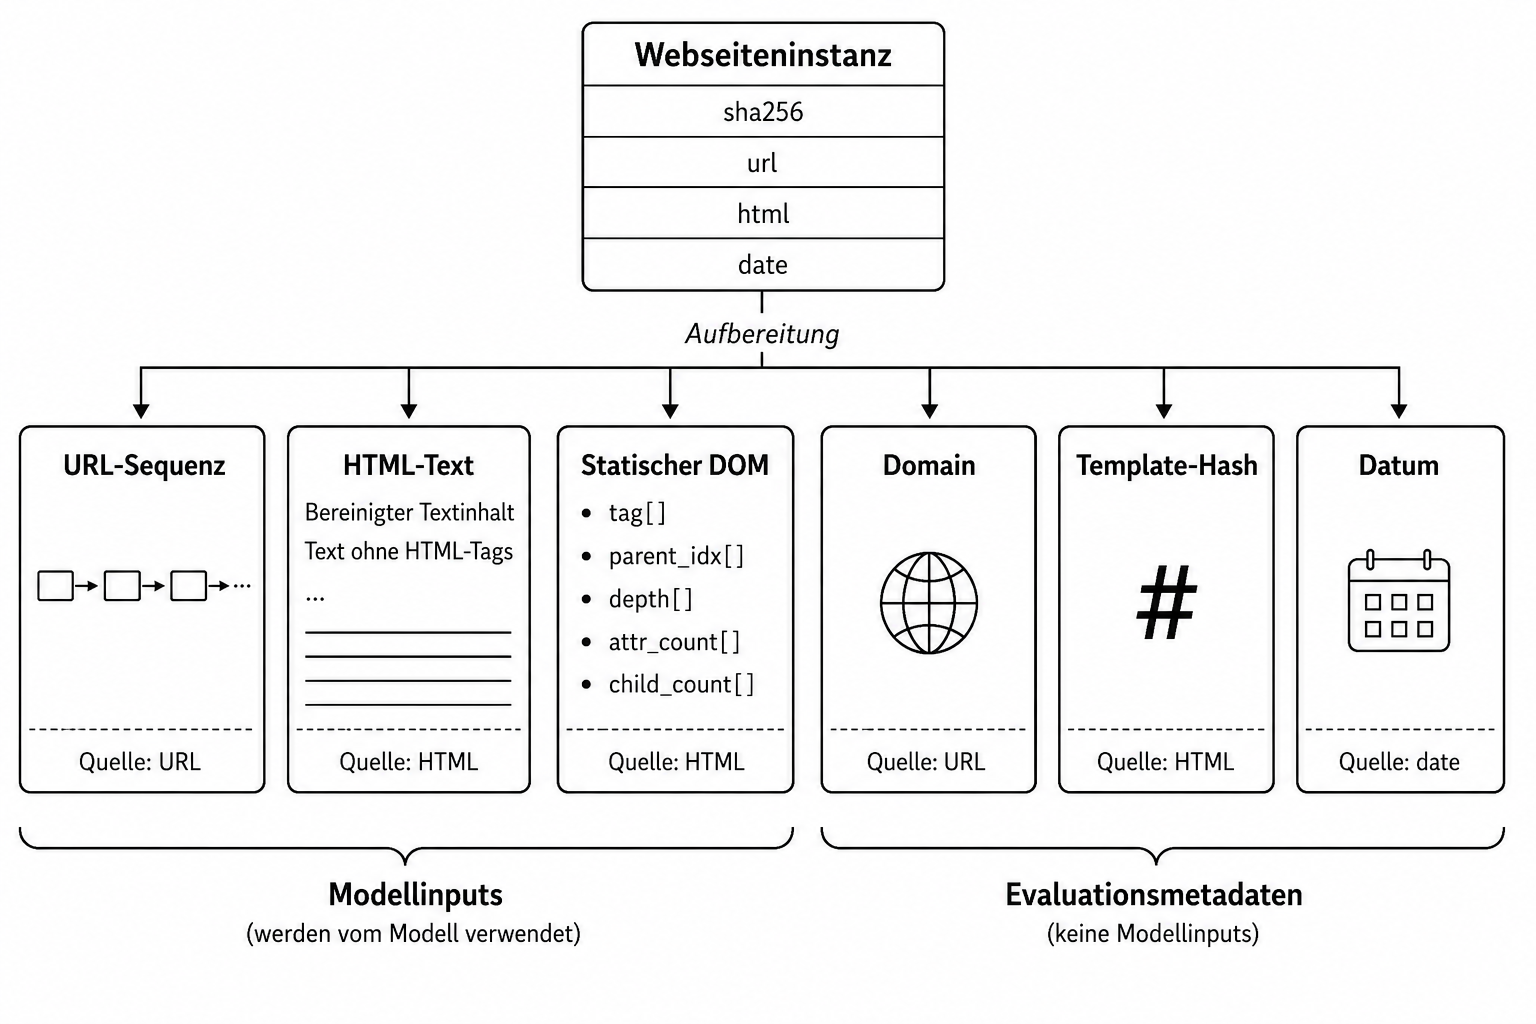
\includegraphics[width=0.85\linewidth]{Praefix/Image/InformationDia.png}
    \caption{Ableitung der Informationsmodalitäten und Evaluationsmetadaten aus einer Webseiteninstanz}
    \label{fig:datenaufbereitung}
{\footnotesize Eigene Darstellung; KI-unterstützt.}
\end{figure}

Aus jeder Webseiteninstanz werden drei Modellinputs und drei Evaluationsmetadaten abgeleitet.
Die URL bleibt als sequenzielle Eingabe erhalten. Aus dem gespeicherten HTML werden ein
bereinigter HTML-Text und ein statischer DOM erzeugt. Für den Text werden Kommentare sowie
Script-, Style-, Noscript- und Template-Bereiche entfernt, anschließend HTML-Tags entfernt,
HTML-Zeichenreferenzen aufgelöst und Whitespace normalisiert. Für den DOM wird das
HTML-Dokument als Baum geparst; pro Knoten werden Tagname, Elternindex, Tiefe,
Attributanzahl und Anzahl direkter Kindknoten gespeichert. Es handelt sich um einen aus dem
gespeicherten HTML rekonstruierten statischen DOM und nicht um einen browserseitig
gerenderten Laufzeit-DOM.
Domain, Template-Hash und Datum werden getrennt davon ausschließlich für die spätere
Evaluation aufbewahrt. Die Domain wird aus der URL bestimmt; der Template-Hash entsteht aus
der normalisierten Folge öffnender und schließender HTML-Tags. Diese drei Größen gehen nicht
als Modellmerkmale in die Klassifikation ein. Abbildung~\ref{fig:datenaufbereitung} fasst die
Trennung von Modellinputs und Evaluationsmetadaten zusammen.

\section{Repräsentations- und Versuchsdesign}

\subsection{Task-adaptive Repräsentationen R0, RU, RT und RUT}

Zur isolierten Untersuchung der task-adaptiven Anpassung wird ein faktorielles
$2\times2$-Design für URL und HTML-Text verwendet. Für jede Modalität stehen der bereits
allgemein selbstüberwacht vortrainierte Basisencoder und eine mittels Masked Language Modeling
auf den ungelabelten Webseitendaten weitertrainierte Variante zur Verfügung. R0 ist damit
keine ``No-SSL''-Bedingung, sondern der nicht zusätzlich task-adaptiv angepasste Ausgangspunkt.
R0 kombiniert BERT Base und RoBERTa Base, RU ausschließlich den angepassten URL-Encoder,
RT ausschließlich den angepassten HTML-Text-Encoder und RUT beide angepassten Encoder.
BERT und RoBERTa bilden festgelegte Ausgangsmodelle ihrer jeweiligen Modalität; untersucht
wird nicht ihre gegenseitige Überlegenheit, sondern der zusätzliche Adaptationsschritt.

Für die Downstream-Analyse werden URL und HTML-Text getrennt encodiert und die Hidden
States unter Berücksichtigung der Attention Mask jeweils zu einer mittleren
Sequenzrepräsentation aggregiert. Die beiden 768-dimensionalen Vektoren werden zu einer für
alle vier Varianten identischen 1.536-dimensionalen Darstellung konkateniert. DOM-Verarbeitung
und multimodale Fusion bleiben in diesem Versuchsblock unberücksichtigt.

\begin{figure}[H]
\centering
\small
\setlength{\tabcolsep}{3pt}
\renewcommand{\arraystretch}{1.18}
\begin{tabular}{p{0.17\textwidth}|p{0.32\textwidth}|p{0.32\textwidth}}
& \centering\textbf{HTML-Text: Basisencoder} & \centering\arraybackslash\textbf{HTML-Text: TAPT-Encoder} \\
\hline
\centering\textbf{URL:\\Basisencoder}
& \centering \fbox{\parbox[c][1.8cm][c]{0.27\textwidth}{\centering\textbf{R0}\\URL: BERT Base\\Text: RoBERTa Base}}
& \centering\arraybackslash \fbox{\parbox[c][1.8cm][c]{0.27\textwidth}{\centering\textbf{RT}\\URL: BERT Base\\Text: RoBERTa TAPT}} \\
\centering\textbf{URL:\\TAPT-Encoder}
& \centering \fbox{\parbox[c][1.8cm][c]{0.27\textwidth}{\centering\textbf{RU}\\URL: BERT TAPT\\Text: RoBERTa Base}}
& \centering\arraybackslash \fbox{\parbox[c][1.8cm][c]{0.27\textwidth}{\centering\textbf{RUT}\\URL: BERT TAPT\\Text: RoBERTa TAPT}} \\
\end{tabular}
\vspace{0.5em}

Alle Varianten: URL-Repräsentation + HTML-Text-Repräsentation $\rightarrow$
1.536-dimensionale Downstream-Darstellung
\caption{Faktorielles Design der task-adaptiven Repräsentationsvarianten}
\label{fig:tapt_design}
{\footnotesize Eigene Darstellung; KI-unterstützt.}
\end{figure}

\subsection{Downstream-Probes, Labelbudgets und Referenzverfahren}

Zur Bewertung der Repräsentationen werden eine logistische Regression als Linear Probe und ein
kleines Mehrschicht-Perzeptron als nichtlineare Probe eingesetzt. Die Transformer-Encoder
bleiben dabei eingefroren. Die Linear Probe misst die unmittelbare lineare Nutzbarkeit der
Repräsentationen für die Zielklassifikation (vgl. [Chen et al. (2020), PDF-S. 3]). Innerhalb einer
Wiederholung erhalten R0, RU, RT und RUT identische gelabelte Trainingsinstanzen und denselben
Downstream-Versuchsaufbau.

Die Downstream-Supervision wird über sieben verschachtelte Budgets von 2.000 bis 200.000
gelabelten Webseiten variiert. Die vollständigen Lernkurven werden mit fünf gepaarten
Wiederholungen bestimmt; für den zentralen Vergleich RUT gegen R0 bei 20.000 Labels wird auf
zehn Paare erweitert. Die TAPT-Checkpoints werden dabei nicht neu trainiert, sodass N10 die
Variation der Labelauswahl und des Downstream-Trainings bei festen Repräsentationen erfasst.
Die Budgets unter 200.000 enthalten je zur Hälfte beide Klassen und sind innerhalb einer
Wiederholung ineinander verschachtelt. Bei 200.000 wird dagegen der vollständige SSL-Bestand
mit 101.578 benignen und 98.422 Phishing-Instanzen verwendet. Die Auswahl benötigt somit
Klasseninformationen, obwohl diese beim vorgelagerten TAPT nicht eingelesen werden. FF3 nutzt dasselbe Budgetraster für den Vergleich mit R0@200k als interner Referenz sowie einer
mit 200.000 Labels trainierten TF-IDF/XGBoost-Pipeline. Da sich bei letzterer zugleich
Repräsentation und Klassifikator ändern, wird dieser Vergleich nur als verfahrensübergreifende
Referenz interpretiert. Ergänzend wird die Label-Effizienz von R0 und RUT auf dem unabhängig
erhobenen Phishing Website Dataset von Putra (2023) geprüft. Der Datensatz wird anhand des
Erfassungszeitpunkts in einen früheren Trainings- und einen späteren Testbestand getrennt. Auf
dem früheren Bestand werden für beide Repräsentationen identische, verschachtelte Budgets von
200, 500, 1.000 und 2.000 gelabelten Webseiten mit zehn gepaarten Linear-Probes verwendet.
Primärer Endpunkt ist die über die logarithmierten Labelbudgets integrierte
Average-Precision-Lernkurve (AP-AULC).

Für Putra werden 10.391 vollständige Datensätze nach Erfassungszeitpunkt geordnet.
Der Schnitt am empirischen 75-\%-Quantil (7. April 2023, 03:33:03,372 UTC) ergibt
7.793 frühere Instanzen (3.554 benign, 4.239 Phishing) und 2.598 spätere Instanzen
(1.686 benign, 912 Phishing); exakte URL-Überschneidungen zwischen beiden Teilen
wurden nicht gefunden. Verarbeitet werden die URL und das bereitgestellte Textmerkmal,
kein neu gerendertes HTML. Die externen Auswertungen sind nachträgliche Transferanalysen.
In einem zusätzlichen Vergleich werden beide Quell-RUT-Encoder über eine MLM-Epoche
auf dem ungelabelten frühen Putra-Pool angepasst (E1); E0 behält die Quell-RUT-Encoder bei.
Beide verwenden dieselben zehn Labelauswahlen und das unveränderte externe Testset.
Der zusätzliche MLM-Schritt verwendet 15\,\% Maskierung, Lernrate $5\cdot10^{-5}$,
Weight Decay 0,01 und 6\,\% Warmup. Das spätere Putra-Testset wird hierfür nicht verwendet.

Ein früherer explorativer Versuchsblock untersucht ergänzend kontrastive Repräsentationen.
R2C und R3C kombinieren modalitätsinterne Ansichten mit URL--HTML-Positivpaaren, während
CSAME nur modalitätsinterne Paare nutzt; Domain- und Template-Identitäten werden aus den
Negativmengen ausgeschlossen. Da dieser Block nicht unter dem finalen R0/RU/RT/RUT-Protokoll
wiederholt wurde, erfolgt ausschließlich eine deskriptive Einordnung anhand der
zugehörigen eigenen Ergebnisartefakte.

\section{Evaluations- und Statistikdesign}

\subsection{Kalibration und Evaluationsbedingungen}

Für die schwellenwertabhängige FINAL-Evaluation wird CAL mit 50.000 ausschließlich legitimen
Webseiten verwendet. Für jede zu bewertende Modell- und Wiederholungskonfiguration wird auf
diesen benignen Instanzen ein Schwellenwert für eine Ziel-False-Positive-Rate von 0,5\,\%
bestimmt. Dieser Wert ist ein festgelegter restriktiver Betriebspunkt der vorliegenden
Untersuchung und kein allgemeiner Standard für Phishing-Erkennungssysteme. Der auf CAL
bestimmte Schwellenwert wird unverändert auf den vollständigen Finalbestand und die daraus
gebildeten Bedingungen übertragen.

\begin{table}[htbp]
\centering
\small
\setlength{\tabcolsep}{4pt}
\renewcommand{\arraystretch}{1.12}
\caption{Evaluationsbedingungen der abschließenden Generalisierungsbewertung.}
\label{tab:testszenarien}
\begin{tabular}{p{0.24\textwidth}p{0.55\textwidth}r}
\hline
\textbf{Bedingung} & \textbf{Operationalisierung} & \textbf{Umfang} \\
\hline
Official Test & Vollständiger offizieller Testbestand & 168.060 \\
Domain-OOD & Domain zuvor nicht in den entwicklungszugänglichen Datenrollen beobachtet & 115.917 \\
Template-OOD & Template-Hash zuvor nicht in den entwicklungszugänglichen Datenrollen beobachtet & 161.223 \\
Domain+Template-OOD & Weder Domain noch Template-Hash zuvor beobachtet & 110.095 \\
Late Test Q4 & Erfassungsdatum ab dem 75-\%-Quantil des Finalbestands & 46.784 \\
\hline
\end{tabular}
\end{table}

Die Zeitbedingung beginnt am 28.10.2025, dem 75-\%-Quantil der Erfassungsdaten.
Wegen gleicher Datumswerte an der Grenze umfasst sie 46.784 Fälle und damit mehr als
genau ein Viertel des Finalbestands.

Zur zusätzlichen Absicherung der Szenariodefinition wurde ein metadatenbasierter
Integritätsaudit durchgeführt. Die exakten Domain- und \nolinkurl{template_hash}-Identitäten der
FINAL-Szenarien wurden hierzu mit SUP, DEV, CAL und dem 200.000 Instanzen umfassenden
SSL/TAPT-Pool abgeglichen. Für alle prüfbaren Domain-OOD- und Template-OOD-Instanzen
ergab sich keine einzige exakte Überschneidung; dies gilt ebenso für das kombinierte
Domain+Template-OOD-Szenario. Für die vorhandenen Identitätswerte weist der Audit somit keine Exposition gegenüber den
geprüften Lernrollen nach; dies bezieht sich auf exakte Identitäten und den archivierten Freeze. Für 1,34\,\% der Domain-OOD-Instanzen beziehungsweise 1,38\,\% im
kombinierten Szenario lag kein auswertbarer Domainwert vor; semantische Ähnlichkeiten oder
Near-Duplicates werden in dieser Arbeit nicht geprüft.

\subsection{Statistische Entscheidungsregeln}

Bei gepaarten Repräsentations- und Architekturvergleichen bildet die jeweilige
Trainingsreplikation die statistische Einheit. Als Effektgröße wird die mittlere Differenz der TPR
in Prozentpunkten berichtet. Für mittlere Paardifferenzen wird das zweiseitige t-Intervall
$\bar d\pm t_{0{,}975;n-1}s_d/\sqrt n$ verwendet; es beschreibt die
Downstream-Variation bei festen Vortrainingszuständen und fester Testpopulation.
Die t-Intervalle setzen unabhängige, näherungsweise normalverteilte Paardifferenzen voraus;
die Sign-Flip-Tests benötigen unter der jeweiligen Nullhypothese Vorzeichensymmetrie.
Die vollständige Enumeration allein macht einen Test nicht voraussetzungsfrei.
Ergänzend werden die Anzahl der
Replikationen mit positiver beziehungsweise negativer Differenz angegeben. Für gepaarte
Vergleiche wird der exakte Sign-Flip-Permutationstest verwendet (vgl. [Holt und Sullivan (2023), S. 787--788]). Mehrere gemeinsam geprüfte Hypothesen werden mit der Holm-Prozedur für
multiples Testen korrigiert (vgl. [Holm (1979), S. 66--67]). Der N10-Vergleich von RUT20k und R020k verwendet \nolinkurl{OFFICIAL_TEST} als primären
Endpunkt. Die vier zusätzlichen domain-, template- und zeitbezogenen Bedingungen bilden eine
gemeinsame sekundäre Testfamilie; ihre vier p-Werte werden innerhalb dieses Vergleichs nach
Holm korrigiert.

Für FF3 wird eine Nichtunterlegenheitsmarge von einem Prozentpunkt TPR festgelegt. Gegen
R0@200k wird für jedes Budget und jede Evaluationsbedingung ein exakter einseitiger
Sign-Flip-Test auf die um diese Marge verschobene gepaarte Differenz berechnet. Ein Budget
gilt nur dann als ausreichend, wenn die Nichtunterlegenheit in allen fünf Bedingungen
gleichzeitig erreicht wird. Der gemeinsame p-Wert ist das Maximum der fünf
Komponenten-p-Werte (Intersection-Union-Prinzip). Anschließend werden die sieben Budgetentscheidungen mit der
Holm-Prozedur korrigiert. Die Marge von einem Prozentpunkt dient als Entscheidungsschwelle
dieser Untersuchung und stellt keine fachlich oder betrieblich validierte Servicegrenze dar. Für den Vergleich von RUT+Linear mit TF-IDF/XGBoost@200k besteht keine natürliche
Paarung der zehn Modellläufe. Deshalb werden die Beobachtungen nicht nachträglich einander
zugeordnet. Dieser nachträgliche Welch-Vergleich wird als ergänzende, verfahrensübergreifende
Evidenz interpretiert. Stattdessen wird für jede Evaluationsbedingung ein einseitiger
Welch-Nichtunterlegenheitstest mit derselben Marge berechnet. 

Auch hier muss die
Nichtunterlegenheit in allen fünf Bedingungen erreicht werden; anschließend werden die sieben
Budgetentscheidungen nach Holm korrigiert. Zusätzlich wird deskriptiv ausgewiesen, ab welchem Budget die mittlere TPR von RUT in allen
fünf Bedingungen mindestens der XGBoost-TPR entspricht und die mittlere FPR gleichzeitig
nicht höher liegt. Diese zusätzliche Auswertung beschreibt ausschließlich die beobachteten
Mittelwerte und stellt keinen Signifikanztest dar.

Da die Nichtunterlegenheitsmarge von einem Prozentpunkt für diese Untersuchung festgelegt
wurde, wird nach Abschluss der primären FF3-Auswertung ergänzend geprüft, wie stark die
ermittelte Budgetstufe von dieser Festlegung abhängt. Hierzu wird dasselbe N10-Protokoll
zusätzlich mit TPR-Margen von 0,0, 0,5 und 2,0 Prozentpunkten ausgewertet. Gegen R0@200k
bleiben der gepaarte einseitige Sign-Flip-Test, die gleichzeitige Bedingung über alle fünf
Evaluationsbedingungen und die Holm-Korrektur über sieben Budgets unverändert. Für
TF-IDF/XGBoost@200k wird analog mit den einseitigen Welch-Tests verfahren. Bei einer
Marge von 0,0 Prozentpunkten wird kein TPR-Nachteil zugelassen; die Entscheidung verlangt
damit einen über alle fünf Bedingungen positiven Unterschied im verwendeten Testprotokoll. Die Sensitivitätsanalyse wurde nach der primären 1-pp-Auswertung ergänzt. Sie dient
ausschließlich dazu, die Stabilität der resultierenden Budgetstufe gegenüber alternativen Margen
zu prüfen. Die 1-pp-Marge bleibt die vorab verwendete Hauptentscheidung und wird durch die
ergänzende Auswertung nicht nachträglich ersetzt.

\section{Konzeption des prototypischen Klassifikationssystems}

\subsection{Zielbild und Gesamtarchitektur}



Aufbauend auf der Repräsentationsanalyse wird ein mehrzweigiges prototypisches
Klassifikationssystem konzipiert. Die DUAL-Variante verarbeitet URL und HTML-Text in
getrennten Transformerzweigen. Die TRI-Variante ergänzt zusätzlich die strukturelle
DOM-Repräsentation. Die Ausgaben der aktiven Modalitäten werden jeweils in einen gemeinsamen
256-dimensionalen Raum projiziert und L2-normalisiert. Eine lernbare Gating-Komponente
bestimmt instanzabhängige Modalitätsgewichte; daraus wird eine gewichtete
Fusionsrepräsentation gebildet. Die Verwendung lernbarer, über Softmax normalisierter
Modalitätsgewichte entspricht dem Prinzip einer gewichteten multimodalen Fusion
(vgl. [Zhou et al. (2019), PDF-S. 2]). 
Für die abschließende Klassifikation werden die einzelnen
Modalitätsrepräsentationen gemeinsam mit der Fusionsrepräsentation verwendet.
Modalitätsspezifische Auxiliary Heads erzeugen zusätzliche Hilfsscores, ohne die
Gating-Gewichte zu ersetzen. Der URL-Hilfsscore bildet zugleich die Grundlage der
URL-first-Kaskade. Die Gesamtarchitektur und die Rollen von DUAL, TRI, Auxiliary Heads,
Gating und Main Head sind in Abbildung~\ref{fig:systemkonzeption} dargestellt. Die technische
Parametrisierung der Encoderfreigabe, DOM-GCN-, Gating- und Head-Komponenten wird erst
in Kapitel 5 spezifiziert. Die Architektur trennt damit drei Ebenen: die Repräsentationsbildung innerhalb der
Modalitätszweige, deren gemeinsame Fusion und die nachgelagerte Klassifikation. Ob jede
zusätzliche Systemkomponente gegenüber einer einfacheren Vorstufe einen eigenen Beitrag
liefert, wird nicht aus dem Endmodell abgeleitet, sondern in einer gesonderten sequenziellen
Ablation geprüft.

\begin{figure}[H]
    \centering
    \makebox[\textwidth][c]{%
        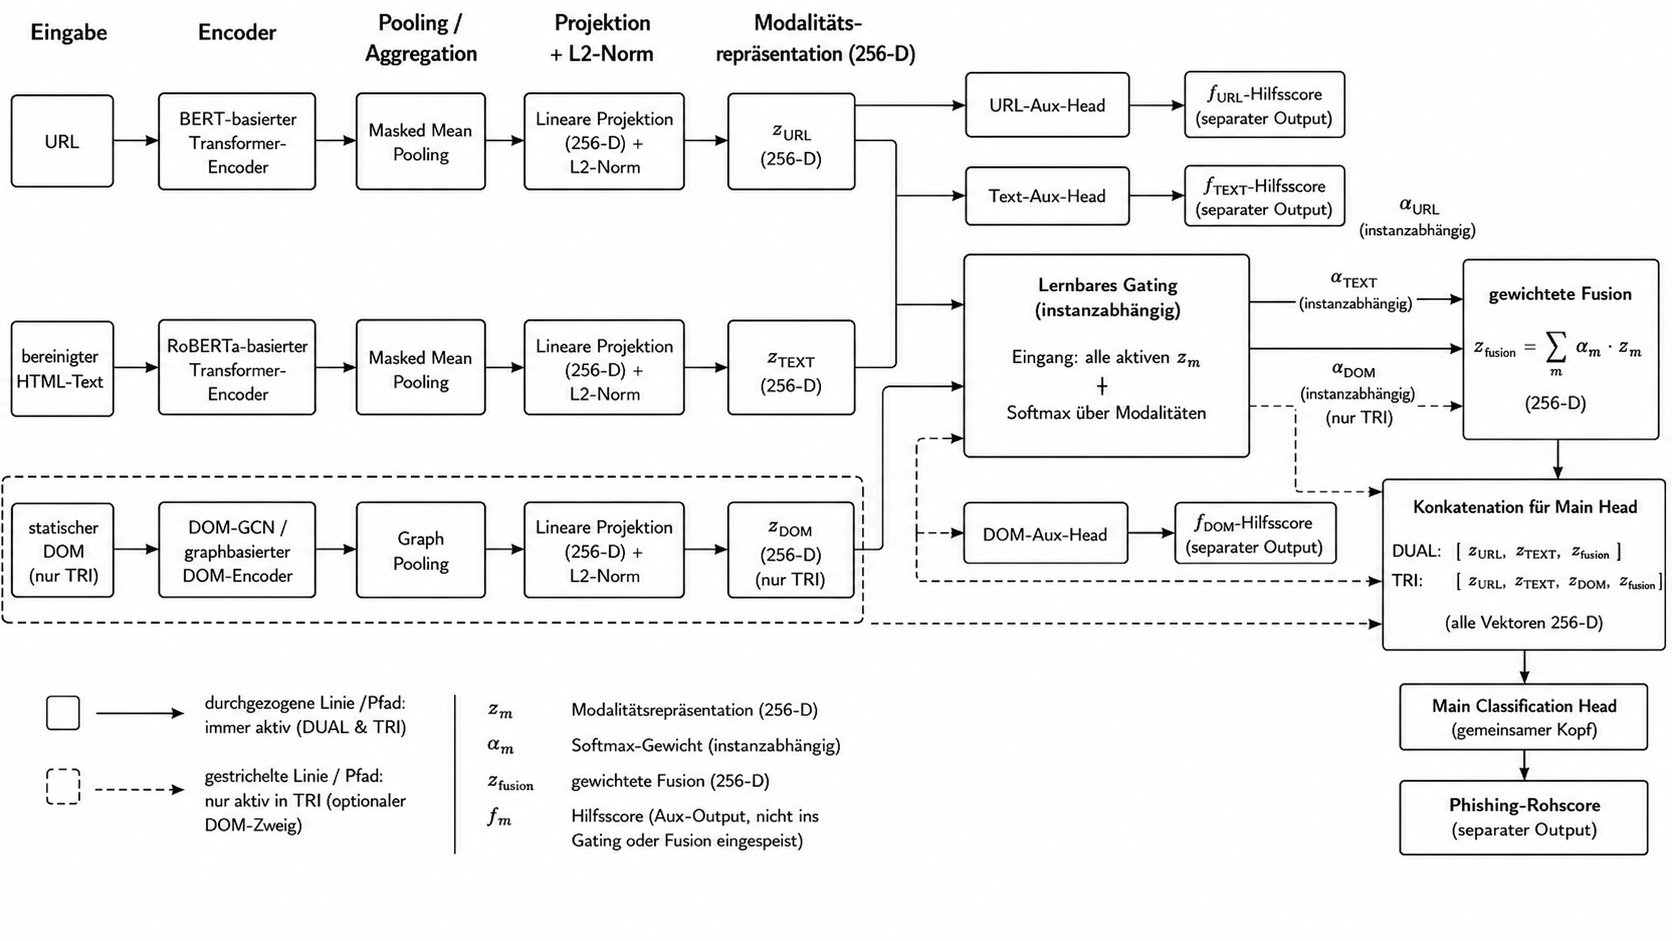
\includegraphics[width=1.0\textwidth]{Praefix/Image/Systemkonzeption.png}%
    }
    \caption{Gesamtarchitektur des prototypischen Klassifikationssystems}
    \label{fig:systemkonzeption}
    \vspace{0.2em}
{\footnotesize Eigene Darstellung; KI-unterstützt.}
\end{figure}

\subsection{Sequenzielle Komponentenablation}

Zur kontrollierten FF4-Komponentenprüfung wird die RUT-Repräsentationsbasis festgehalten und
vier verschachtelte Systemvarianten werden verglichen:
\[
\begin{aligned}
P_0&=\text{URL}, &
P_1&=\text{URL+Text, Equal},\\
P_2&=\text{URL+Text+DOM, Equal}, &
P_3&=\text{URL+Text+DOM, Gated}.
\end{aligned}
\]

Damit quantifiziert $P_1-P_0$ den zusätzlichen Textbeitrag, $P_2-P_1$ den zusätzlichen
DOM-Beitrag und $P_3-P_2$ den Beitrag der lernbaren Gating-Fusion. Die vier Varianten
werden mit zehn gepaarten Replikationen auf derselben balancierten Stichprobe aus
20.000 Labels trainiert. Die initialen RUT-URL- und Textcheckpoints sowie der DOM-SSL-Encoder bleiben
identisch; die freigegebenen Modellparameter werden überwacht trainiert. Für alle Varianten werden eine Epoche und Batchgröße acht verwendet. Die Komponentenablation verwendet ausschließlich Development-Daten. Der Schwellenwert wird
auf den benignen Beispielen der Teilmenge \nolinkurl{ENG_TUNE} bei einer Ziel-FPR von
0,5\,\% bestimmt. Primärer Endpunkt der Komponentenablation ist die TPR auf der von
\nolinkurl{ENG_TUNE} getrennten Teilmenge \nolinkurl{ENG_META}. CAL und FINAL werden für
diese Analyse nicht verwendet. Für die drei benachbarten N10-Vergleiche werden exakte
zweiseitige Sign-Flip-Tests berechnet und gemeinsam nach Holm korrigiert.

\subsection{URL-first-Kaskade und Frontend-Vergleich}

\begin{figure}[H]
    \centering
    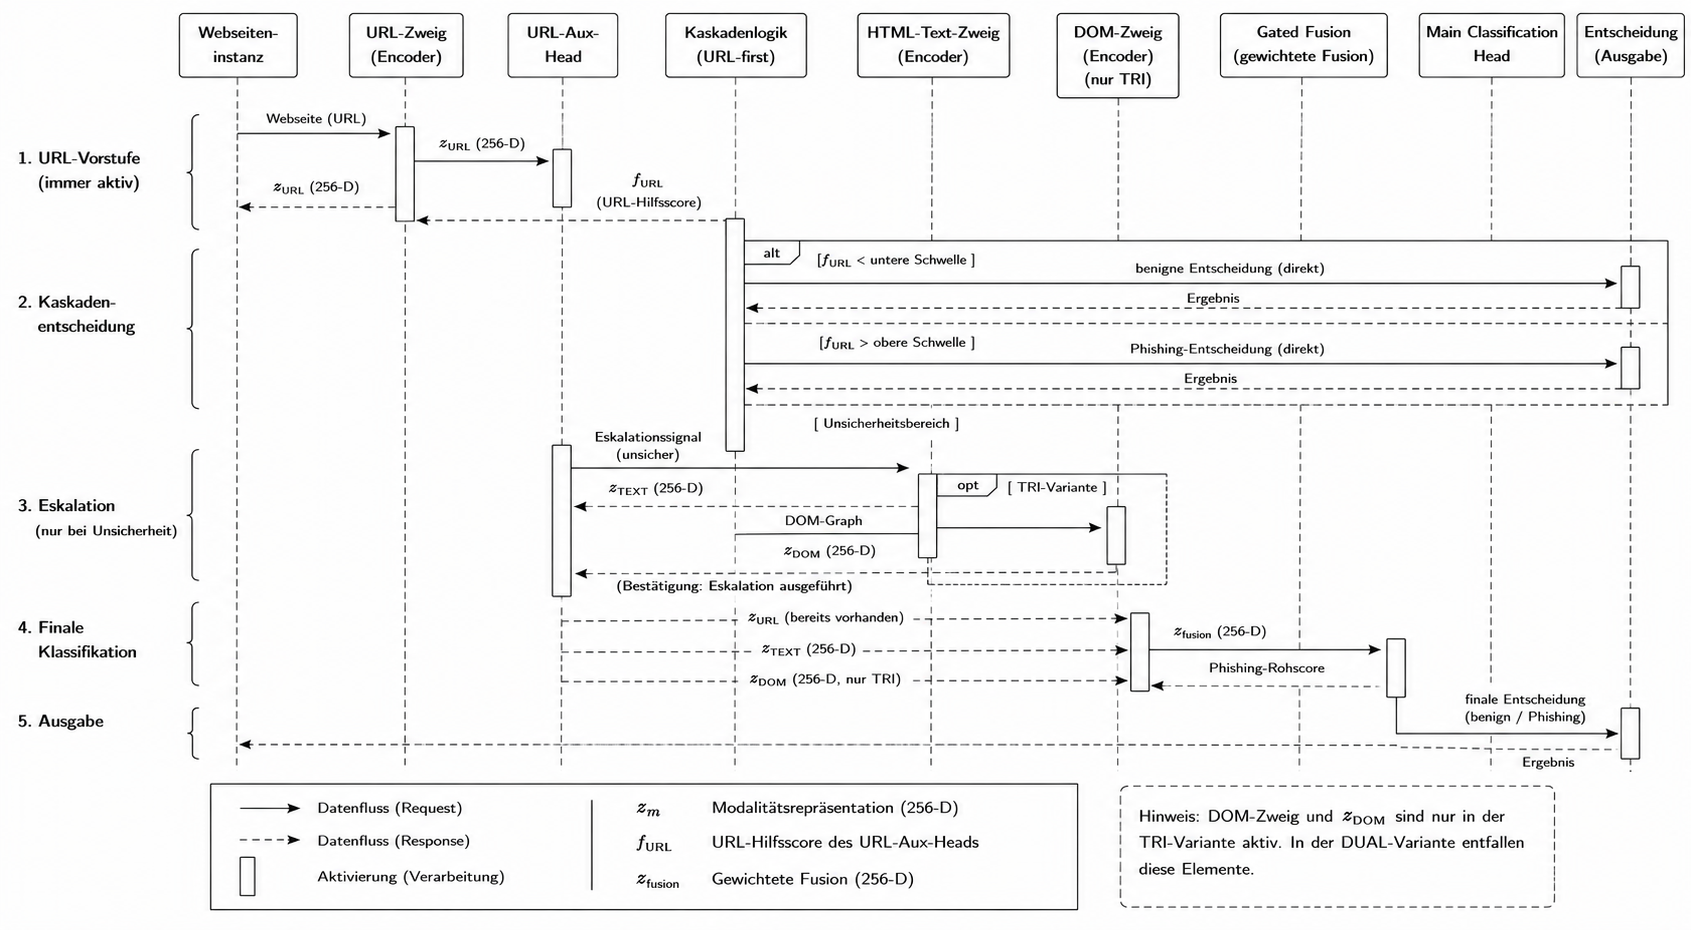
\includegraphics[width=1\linewidth]{Praefix/Image/URLKaskade.png}
    \caption{Sequenzdiagramm der bedingten Verarbeitung in der URL-first-Kaskade}
    \label{fig:urlkaskade}
{\footnotesize Eigene Darstellung; KI-unterstützt.}
\end{figure}

Die URL-first-Kaskade führt zunächst ausschließlich den URL-Zweig aus und erzeugt über den
URL-Auxiliary-Head den Score $f_{\mathrm{URL}}$. Eine untere und eine obere, auf
Development-Daten bestimmte Schwelle begrenzen einen Unsicherheitsbereich. Liegt der Score
außerhalb dieses Bereichs, wird die Klassifikation bereits nach dem URL-Pfad abgeschlossen.
Nur die dazwischenliegenden Fälle durchlaufen zusätzlich den vollständigen multimodalen Pfad.
Dieses Vorgehen entspricht dem Grundprinzip kaskadierter Klassifikatoren
(vgl. [Viola und Jones (2004), S. 144--145]). Bei einer Eskalation wird die bereits berechnete URL-Repräsentation wiederverwendet und um
HTML-Text sowie in der TRI-Variante um den DOM ergänzt. Die aktiven Repräsentationen
durchlaufen anschließend dieselbe Fusion und denselben Klassifikationskopf wie im Vollsystem.
Abbildung~\ref{fig:urlkaskade} zeigt den Ablauf und verdeutlicht, dass der DOM-Zweig nur für
eskalierte TRI-Fälle ausgeführt wird. Zusätzlich wird untersucht, ob die verwendete URL-Repräsentation den Anteil der Eskalationen
beeinflusst. TRI-Fallback, Labelbudget und grundsätzliche Routinglogik bleiben hierfür
unverändert; variiert wird ausschließlich zwischen der Basis- und der task-adaptierten
URL-Repräsentation. Die Routingparameter werden auf Development-Daten für zulässige
TPR-Abweichungen von 0,25, 0,5, 1,0 und 2,0 Prozentpunkten gegenüber dem Vollsystem
bestimmt. Die primär betrachtete Toleranz beträgt einen Prozentpunkt. Als zentrale
Ressourcenkennzahl wird die Eskalationsrate berichtet, also der Anteil der Webseiten, für die
der vollständige multimodale Pfad ausgeführt wird. Verglichen wird damit der erforderliche
Verarbeitungsumfang unter derselben vorgegebenen TPR-Toleranz.

\section{Freeze, Reproduzierbarkeit und Grenzen des Untersuchungsdesigns}

Die ursprüngliche Repräsentations- und Systementwicklung erfolgt auf den vorgesehenen
Development-Daten; vor dem Zugriff auf CAL und FINAL wird für den finalen Integrationslauf
ein Architecture-Freeze gespeichert. CAL wird danach ausschließlich zur Schwellenwertbestimmung
verwendet, während FINAL und die daraus gebildeten Teilmengen ausschließlich der abschließenden
Leistungsbewertung dienen. Datenrollen, Modellzustände, Konfigurationen, Seeds und
Auswertungsartefakte werden gespeichert sowie die Disjunktheit der Datenrollen, die erwarteten
Instanzzahlen und die Vollständigkeit der Ergebnisartefakte automatisiert geprüft.

Mehrere ergänzende Analysen wurden erst nach Vorliegen früherer Ergebnisse durchgeführt.
Der Vergleich mit TF-IDF/XGBoost wurde nach den ersten RUT/R0-Ergebnissen um das
vollständige Budgetraster von 2.000 bis 200.000 Labels erweitert; sämtliche sieben
Budgetstufen werden berichtet und der Analyseplan wurde vor der Ausführung gespeichert.
Auch die sequenzielle FF4-Komponentenablation wurde erst nach Festlegung der finalen
Architektur ergänzt. Varianten, neue Seeds, die drei Komponentenvergleiche und die
Schwellenlogik wurden vor ihrer Durchführung festgelegt, während CAL und FINAL weiterhin
ausgeschlossen blieben. Die Komponentenablation dient damit der nachträglichen Prüfung der
bereits festgelegten Systembestandteile und nicht der erneuten Auswahl der finalen Architektur. Die Sensitivitätsanalyse der FF3-Marge wurde nach Abschluss der primären 1-pp-Auswertung
ergänzt und wendet ohne erneutes Modelltraining dieselben statistischen Entscheidungsregeln
auf alternative Margen von 0,0, 0,5 und 2,0 Prozentpunkten an. Sie prüft ausschließlich, ob
sich die kleinste ausreichende Budgetstufe bei alternativen Festlegungen verändert. Die
Wiederholungen variieren die Labelauswahl und das Downstream-Training bei unveränderten
Repräsentations- beziehungsweise Pretraining-Checkpoints und erfassen daher nicht die Varianz
vollständig neu ausgeführter selbstüberwachter Vortrainingsläufe. Aussagen zur reduzierten
Labelmenge beziehen sich ausschließlich auf die gelabelte Downstream-Supervision.


Die betriebliche Szenarioanalyse wird nach Abschluss der Modellauswertung ergänzt. Sie
verwendet die eingefrorenen FINAL-Konfusionsmatrizen und klassenspezifischen Routinganteile,
ohne Schwellen neu auszuwählen. Referenzvolumen und Phishinganteile sind ausdrücklich
angenommene Größen. Die Umrechnung setzt unverändertes Fehler- und Routingverhalten
innerhalb beider Klassen voraus; ihre Werte sind bedingte Erwartungswerte ohne zusätzliche
Unsicherheitsintervalle. Der gemessene In-Memory-Durchsatz bleibt eine separate technische
Referenz. Ein betrieblicher Pilot oder ein neuer Verteilungstest wird dadurch nicht ersetzt.

\lstset{
  basicstyle=\ttfamily\small,
  numbers=left,
  numberstyle=\tiny,
  stepnumber=2,
  numbersep=6pt,
  frame=single,
  framerule=0.3pt,
  breaklines=true,
  breakatwhitespace=false,
  breakindent=1.0em,
  columns=fullflexible,
  keepspaces=true,
  showstringspaces=false,
  xleftmargin=2.4em,
  xrightmargin=0.5em,
  aboveskip=0.30\baselineskip,
  belowskip=0.30\baselineskip,
  captionpos=b
}

